\documentclass{beamer}
\usepackage{amsmath, amssymb}
\usepackage{graphicx}
\usepackage{listings}
\usepackage{color}

% Set up R code formatting
\definecolor{codegreen}{rgb}{0,0.6,0}
\definecolor{codegray}{rgb}{0.5,0.5,0.5}
\definecolor{codepurple}{rgb}{0.58,0,0.82}
\definecolor{backcolour}{rgb}{0.95,0.95,0.92}
\lstdefinestyle{Rstyle}{
    backgroundcolor=\color{backcolour},
    commentstyle=\color{codegreen},
    keywordstyle=\color{magenta},
    numberstyle=\tiny\color{codegray},
    stringstyle=\color{codepurple},
    basicstyle=\ttfamily\footnotesize,
    breakatwhitespace=false,
    breaklines=true,
    captionpos=b,
    keepspaces=true,
    numbers=left,
    numbersep=5pt,
    showspaces=false,
    showstringspaces=false,
    showtabs=false,
    tabsize=2
}

\title{Mixed Effects Models - Day 7}
\subtitle{Diagnostics of Mixed Effects Models}
\author{Marieke Wesselkamp\\Department of Biometry and Environmental Systems Analysis\\Albert-Ludwigs-University of Freiburg (Germany)}
\date{February 2023}

\begin{document}

\frame{\titlepage}

\begin{frame}
    \frametitle{The Linear Mixed Effects Model}
    \[
    \mathbf{y} = \mathbf{X} \cdot \mathbf{b} + \mathbf{Z} \cdot \mathbf{u} + \mathbf{e}
    \]
    where:
    \begin{itemize}
        \item $\mathbf{y}$: measured response values
        \item $\mathbf{X}$: Fixed Effects design matrix
        \item $\mathbf{b}$: Fixed Effects parameter vector
        \item $\mathbf{u}$: Random Effects parameter vector, $\mathbf{u} \sim \mathcal{N}(0, \mathbf{G})$
        \item $\mathbf{e}$: Residual errors, $\mathbf{e} \sim \mathcal{N}(0, \mathbf{R})$
    \end{itemize}
\end{frame}

\begin{frame}
    \frametitle{Stochastic Parts of Mixed Effects Models}
    \begin{itemize}
        \item \textbf{Random effects:} 
        \[
        \mathbf{u} \sim \mathcal{N}(0, \mathbf{G})
        \]
        Describes how random effects parameters $\mathbf{u}$ vary around 0.
        
        \item \textbf{Residual variance:} 
        \[
        \mathbf{e} \sim \mathcal{N}(0, \mathbf{R})
        \]
        Unexplained variance after accounting for fixed and random effects.
    \end{itemize}
\end{frame}

\begin{frame}
    \frametitle{Assumptions of Mixed Effects Models}
    \begin{enumerate}
        \item $\mathbf{b}$ describes the deterministic trend averaged over the random effects $\mathbf{u}$.
        \item Random effects $\mathbf{u}$ are normally distributed with mean 0 and covariance matrix $\mathbf{G}$.
        \item Residual errors $\mathbf{e}$ are normally distributed with mean 0 and variance $\sigma^2$.
        \item $\mathbf{u}$ and $\mathbf{e}$ are independent.
        \item Variances and covariances are homogeneous across groups.
    \end{enumerate}
\end{frame}

\begin{frame}
    \frametitle{Checking Model Assumptions}
    Violations of these assumptions can lead to problems with residuals and fitting. Each assumption must be tested.
\end{frame}

\begin{frame}
    \frametitle{Model Specification: Key Components}
    To build a well-behaved model:
    \begin{itemize}
        \item Define the fixed effects part, including interactions and nonlinear terms.
        \item Choose an appropriate error distribution.
        \item Spot the grouping in the data and specify random effects correctly.
    \end{itemize}
\end{frame}

\begin{frame}
    \frametitle{Residual Checks for LMEMs}
    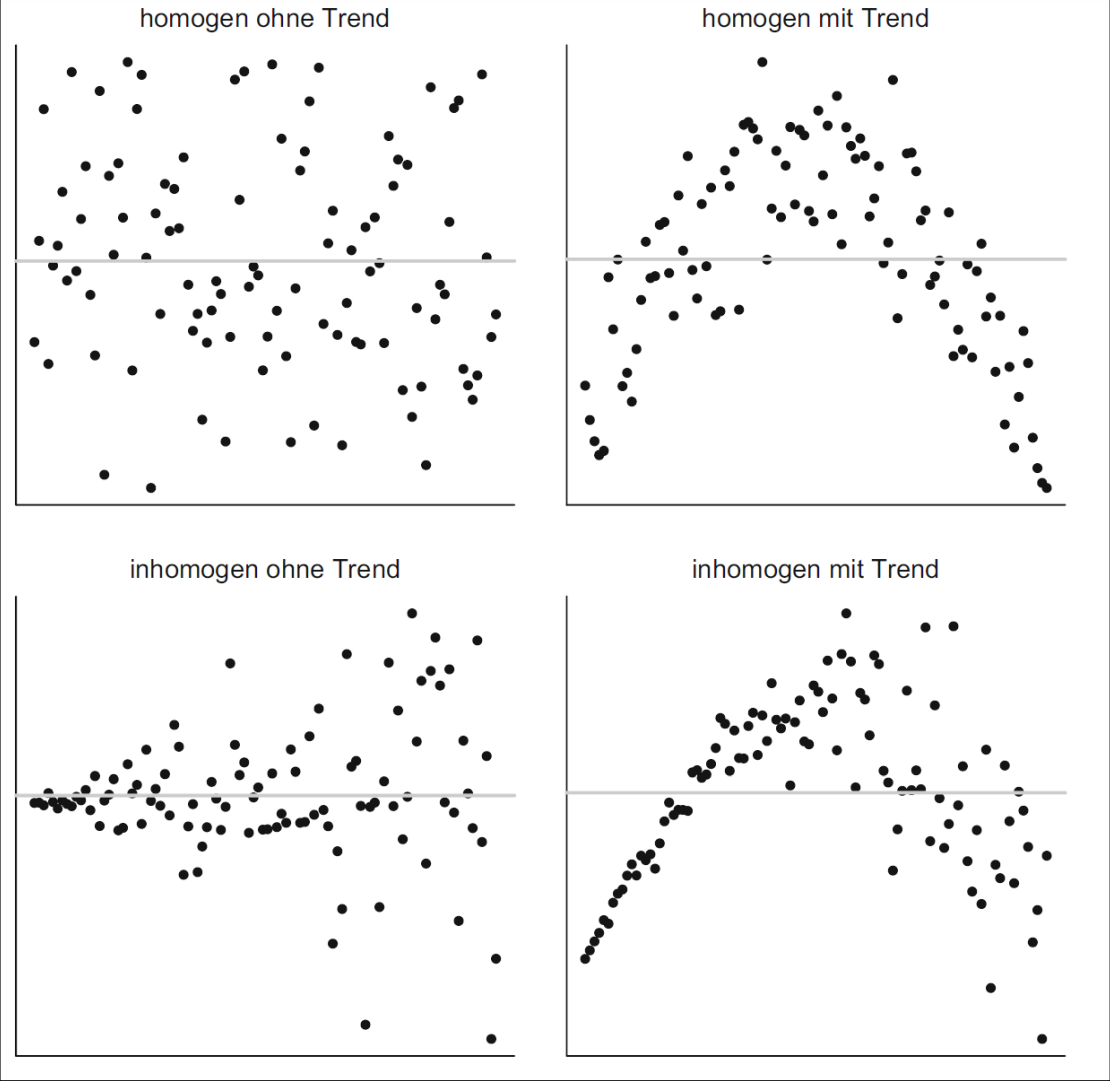
\includegraphics[width=0.45\textwidth]{residuals.png}
    \newline
    Linear Mixed Effects Models (LMEMs) require more checks because they have more assumptions.
\end{frame}

\begin{frame}
    \frametitle{Check the Grouping in the Output}
    Example: Glycogen concentration measurements from a nested design involving rats, livers, and preparation methods.
\end{frame}

\begin{frame}[fragile]
    \frametitle{R Code: Glycogen Data}
    \lstset{style=Rstyle}
    \begin{lstlisting}
    rats <- read.table("rats.txt", header = TRUE)
    rats$prep <- rep(c(1, 2), 18)
    rats$Treatment <- factor(rats$Treatment)
    rats$Rat <- factor(rats$Rat)
    rats$Liver <- factor(rats$Liver)
    rats$prep <- factor(rats$prep)
    \end{lstlisting}
    Nested design with 3 treatments, 2 rats per treatment, 3 liver pieces, and 2 preparations per liver piece.
\end{frame}

\begin{frame}[fragile]
    \frametitle{Plotting Glycogen Data}
    \lstset{style=Rstyle}
    \begin{lstlisting}
    par(mfrow = c(1,1), las = 1)
    plot(rats$Glycogen, ylab = "Glycogen", pch = c(rep(21,6), rep(22,6)), cex = 2)
    \end{lstlisting}
\end{frame}

\begin{frame}[fragile]
    \frametitle{Mixed Effects Model (Nested Design)}
    \lstset{style=Rstyle}
    \begin{lstlisting}
    m.r <- lmer(Glycogen ~ Treatment + (1|Rat/Liver), data = rats)
    summary(m.r)
    \end{lstlisting}
\end{frame}

\begin{frame}[fragile]
    \frametitle{Alternative Model (Crossed Design)}
    \lstset{style=Rstyle}
    \begin{lstlisting}
    m.r.2 <- lmer(Glycogen ~ Treatment + (1|Rat) + (1|Liver), data = rats)
    summary(m.r.2)
    \end{lstlisting}
    Different grouping leads to different variance components.
\end{frame}

\begin{frame}
    \frametitle{Check the Variance Components}
    A high correlation or singular fit may indicate an issue with model specification.
\end{frame}

\begin{frame}[fragile]
    \frametitle{Variance Components Example}
    \lstset{style=Rstyle}
    \begin{lstlisting}
    m.f <- lmer(root ~ week * fertilizer + (week|plant), fertilizer)
    summary(m.f)
    \end{lstlisting}
    \textbf{Singular fit detected:} The model may be over-specified.
\end{frame}

\begin{frame}[fragile]
    \frametitle{Maximizing Random Effects Specification}
    \lstset{style=Rstyle}
    \begin{lstlisting}
    m.f.no <- lmer(root ~ week * fertilizer + (week || plant), fertilizer)
    summary(m.f.no)
    \end{lstlisting}
    Keeping the model as maximal as possible.
\end{frame}

\begin{frame}
    \frametitle{Check Normality of Random Effects}
    Use visual tools such as histograms and QQ plots to check for normality.
\end{frame}

\begin{frame}[fragile]
    \frametitle{Random Intercept Check}
    \lstset{style=Rstyle}
    \begin{lstlisting}
    hist(ranef(m.f.no)$plant[,1])  # Random intercept
    shapiro.test(ranef(m.f.no)$plant[,1])
    \end{lstlisting}
    The Shapiro-Wilk test helps check if the random intercepts are normally distributed.
\end{frame}

\begin{frame}[fragile]
    \frametitle{Random Slope Check}
    \lstset{style=Rstyle}
    \begin{lstlisting}
    hist(ranef(m.f.no)$plant[,2])  # Random slope
    shapiro.test(ranef(m.f.no)$plant[,2])
    \end{lstlisting}
\end{frame}

\begin{frame}[fragile]
    \frametitle{QQ Plots for Random Effects}
    \lstset{style=Rstyle}
    \begin{lstlisting}
    qqmath(ranef(m.f.no)$plant[,1], panel = function(x, ...) {
        panel.qqmathline(x, ...)
        panel.qqmath(x, ...)
    })
    \end{lstlisting}
    \textbf{Intercept} (QQ Plot)
\end{frame}

\begin{frame}[fragile]
    \frametitle{QQ Plots for Random Slope}
    \lstset{style=Rstyle}
    \begin{lstlisting}
    qqmath(ranef(m.f.no)$plant[,2], panel = function(x, ...) {
        panel.qqmathline(x, ...)
        panel.qqmath(x, ...)
    })
    \end{lstlisting}
    \textbf{Slope} (QQ Plot)
\end{frame}

\begin{frame}
    \frametitle{Conclusion}
    \begin{itemize}
        \item Ensure proper grouping and variance components in mixed models.
        \item Use diagnostic tools to check for violations in model assumptions.
        \item Random effects normality checks require sufficient data points to be reliable.
    \end{itemize}
\end{frame}

\begin{frame}[fragile]
    \frametitle{Random Effects Model: Genotype Deviations}
    \lstset{style=Rstyle}
    \begin{lstlisting}
    geno <- read.table("nlme.txt", header = TRUE)
    m.g <- lmer(Height ~ poly(P,2) + (poly(P,2)|Genotype), geno)
    xyplot(Height ~ P | Genotype, geno)
    \end{lstlisting}
\end{frame}

\begin{frame}[fragile]
    \frametitle{Genotype-Specific Deviations}
    \lstset{style=Rstyle}
    \begin{lstlisting}
    VarCorr(m.g)
    \end{lstlisting}
    Genotype-specific deviations from the nonlinear population trend.
\end{frame}

\begin{frame}[fragile]
    \frametitle{Distribution of Random Effects}
    \lstset{style=Rstyle}
    \begin{lstlisting}
    hist(ranef(m.g)$Genotype[,1])
    \end{lstlisting}
\end{frame}

\begin{frame}
    \frametitle{Check Your Residuals}
    Revisiting the Orthodont dataset for residual checks.
\end{frame}

\begin{frame}[fragile]
    \frametitle{Plotting Residuals: Orthodont Data}
    \lstset{style=Rstyle}
    \begin{lstlisting}
    data(Orthodont, package = "nlme")
    attach(Orthodont)
    fm1 <- lmer(distance ~ age * Sex + (age | Subject))
    plot(fm1)
    \end{lstlisting}
    No strong visible trend, but further investigation is needed.
\end{frame}

\begin{frame}[fragile]
    \frametitle{QQ Plot of Residuals}
    \lstset{style=Rstyle}
    \begin{lstlisting}
    require("lattice")
    qqmath(fm1, id = 0.05)
    \end{lstlisting}
    Three data points seem to deviate significantly.
\end{frame}

\begin{frame}
    \frametitle{Residual Plotting Strategy}
    An overall plot might mask issues, so it is important to subset the residuals in meaningful ways.
\end{frame}

\begin{frame}[fragile]
    \frametitle{Standardized Residuals vs Age}
    \lstset{style=Rstyle}
    \begin{lstlisting}
    plot(fm1, resid(., scaled = TRUE) ~ age, abline = 0)
    \end{lstlisting}
    Residuals by age, showing potential variance differences across ages.
\end{frame}

\begin{frame}[fragile]
    \frametitle{Response Residuals vs Fitted by Age}
    \lstset{style=Rstyle}
    \begin{lstlisting}
    plot(fm1, resid(.) ~ fitted(.) | age, abline = 0)
    \end{lstlisting}
    Produces residual plots for each age value.
\end{frame}

\begin{frame}[fragile]
    \frametitle{Response Residuals vs Fitted by Sex}
    \lstset{style=Rstyle}
    \begin{lstlisting}
    plot(fm1, resid(.) ~ fitted(.) | Sex, abline = 0)
    \end{lstlisting}
    Shows larger residual spread for boys, indicating a violation of the homogeneous variance assumption.
\end{frame}

\begin{frame}[fragile]
    \frametitle{Modeling Heterogeneous Residual Variance}
    \lstset{style=Rstyle}
    \begin{lstlisting}
    mod <- lme(distance ~ age * Sex, random = ~ age | Subject, weights = varIdent(form = ~ 1 | Sex))
    getVarCov(mod, type = "random.effects")
    \end{lstlisting}
\end{frame}

\begin{frame}[fragile]
    \frametitle{Extracting Conditional Variance-Covariance Matrix}
    \lstset{style=Rstyle}
    \begin{lstlisting}
    getVarCov(mod, individuals = 1, type = "conditional")
    getVarCov(mod, individuals = 27, type = "conditional")
    \end{lstlisting}
\end{frame}

\begin{frame}[fragile]
    \frametitle{Modeling Group-Specific Variance}
    \lstset{style=Rstyle}
    \begin{lstlisting}
    model <- lme(distance ~ age * Sex, random = list(Subject = pdDiag(form = ~ Sex), Subject = pdSymm(form = ~ age)))
    VarCorr(mod)
    VarCorr(model)
    \end{lstlisting}
\end{frame}

\begin{frame}
    \frametitle{Check Residuals on the Random Effects Level}
    Box plots of standardized residuals by Subject.
\end{frame}

\begin{frame}[fragile]
    \frametitle{Residuals by Subject}
    \lstset{style=Rstyle}
    \begin{lstlisting}
    plot(fm1, Subject ~ resid(.))
    \end{lstlisting}
    M09 and M13 (both boys) have much larger variances than other children.
\end{frame}

\begin{frame}[fragile]
    \frametitle{Observed vs Fitted by Subject}
    \lstset{style=Rstyle}
    \begin{lstlisting}
    plot(fm1, distance ~ fitted(.) | Subject, abline = c(0,1))
    \end{lstlisting}
    M09 and M13 show much larger variances than the others.
\end{frame}

\begin{frame}[fragile]
    \frametitle{Standardized Residuals by Age and Subject}
    \lstset{style=Rstyle}
    \begin{lstlisting}
    plot(fm1, resid(.) ~ age | Subject, abline = 0)
    \end{lstlisting}
\end{frame}

\begin{frame}
    \frametitle{Modeling Within-Group Variance}
    One could allow each child their own variance, instead of assuming the same variance within each level.
\end{frame}

\begin{frame}[fragile]
    \frametitle{1. Check for Singularity}
    \lstset{style=Rstyle}
    \begin{lstlisting}
    VarCorr(m.f)
    isSingular(m.f)
    VarCorr(m.f.2)
    isSingular(m.f.2)
    \end{lstlisting}
\end{frame}

\begin{frame}[fragile]
    \frametitle{2. Scale Predictors}
    \lstset{style=Rstyle}
    \begin{lstlisting}
    m.f.scaled <- lmer(root ~ scale(week) * fertilizer + (scale(week) | plant), fertilizer)
    VarCorr(m.f.scaled)
    isSingular(m.f.scaled)
    \end{lstlisting}
\end{frame}

\begin{frame}[fragile]
    \frametitle{3. Specify Starting Values for Parameters}
    \lstset{style=Rstyle}
    \begin{lstlisting}
    a <- getME(m.f, c("theta"))
    b <- getME(m.f, c("beta"))
    m.check <- lmer(root ~ week * fertilizer + (week | plant), start = list(theta = a, fixef = b))
    isSingular(m.check)
    \end{lstlisting}
\end{frame}

\begin{frame}[fragile]
    \frametitle{4. Compare Optimizers}
    \lstset{style=Rstyle}
    \begin{lstlisting}
    modelfit.all <- lme4::allFit(m.f)
    ss <- summary(modelfit.all)
    ss$fixef
    \end{lstlisting}
    Fixed effects are similar across optimizers.
\end{frame}

\begin{frame}
    \frametitle{Residual Simulations}
    - Simulate responses under the postulated model.
    - Repeat the process many times.
    - Create a distribution of simulated residuals and compare to observed residuals.
\end{frame}

\begin{frame}[fragile]
    \frametitle{Residual Simulations with DHARMa}
    \lstset{style=Rstyle}
    \begin{lstlisting}
    library(DHARMa)
    \end{lstlisting}
    \begin{itemize}
        \item DHARMa package documentation: \href{https://cran.r-project.org/web/packages/DHARMa/vignettes/DHARMa.html}{here}.
    \end{itemize}
\end{frame}

\begin{frame}
    \frametitle{Recap of Day 8}
    \begin{itemize}
        \item Diagnose Linear Mixed Effects Models by checking variance components, random effects, and residuals.
        \item Plot residuals for unique random effects levels and consider complex R-side and G-side matrices.
    \end{itemize}
\end{frame}

\end{document}